\chapter{Felhasználói dokumentáció}
\label{ch:user}

\section{A szoftver általános bemutatása}

A kalaha játék applikáció egy klasszikus táblajáték modern, digitális adaptációja. A program három különböző játékmódot kínál: helyi többjátékos módot, online többjátékos módot, valamint AI elleni játék lehetőségét. Az alkalmazás célja, hogy a játékosok számára könnyen hozzáférhető és élvezetes módon tegye elérhetővé ezt az ősi stratégiai játékot.

\subsection{Rendszerkövetelmények}
A program futtatásához az alábbi minimális rendszerkövetelmények szükségesek:
\begin{itemize}
	\item Operációs rendszer: Windows 10 vagy újabb
	\item Processzor: Intel Core i3 vagy jobb
	\item Memória: 4 GB RAM
	\item Grafikus kártya: DirectX 11 kompatibilis
	\item Internet kapcsolat: Online játékhoz stabil internetkapcsolat szükséges
	\item Tárhely: 500 MB szabad terület
\end{itemize}

\subsection{A játék szabályai}
A kalaha egy két személyes stratégiai játék, amelyben a játékosok célja minél több kő összegyűjtése. A játék szabályai:

\begin{enumerate}
	\item A játéktábla 2x6 kisebb gödörből és 2 nagyobb gyűjtőgödörből áll
	\item Minden kis gödörben kezdetben 4 kő található
	\item A játékosok felváltva lépnek
	\item Egy lépés során a játékos kiválaszt egy gödröt a saját oldaláról, és az összes követ egyesével szétosztja az óramutató járásával megegyező irányban
	\item Ha az utolsó kő a saját gyűjtőgödörébe kerül, a játékos újra léphet
	\item Ha az utolsó kő egy üres gödörbe kerül a saját oldalán, a játékos megszerzi ezt a követ és az átellenes gödör köveit is
	\item A játék véget ér, ha az egyik játékos oldalán minden gödör kiürül, ekkor a másik játékos összegyűjti a maradék köveit. A győztes az aki több követ tudott összegyűjteni.
\end{enumerate}

\section{A program használata}

\subsection{Főmenü}
A program indításakor a főmenü jelenik meg, ahol három játékmód közül választhatunk:

\begin{itemize}
	\item \textbf{Többjátékos mód:} Online játék más játékosok ellen
	\item \textbf{Lokális játék:} Helyi játék két játékos részére egy számítógépen
	\item \textbf{AI elleni játék:} Játék a mesterséges intelligencia ellen
\end{itemize}

\subsection{Online játék}
Az online játékmód választása esetén a szoba kezelő felület jelenik meg. Itt lehetőség van:

\begin{itemize}
	\item Meglévő szobák böngészésére és csatlakozásra
	\item Új szoba létrehozására
	\item Csatlakozásra szobakód alapján
\end{itemize}

\begin{figure}[h]
	\centering
	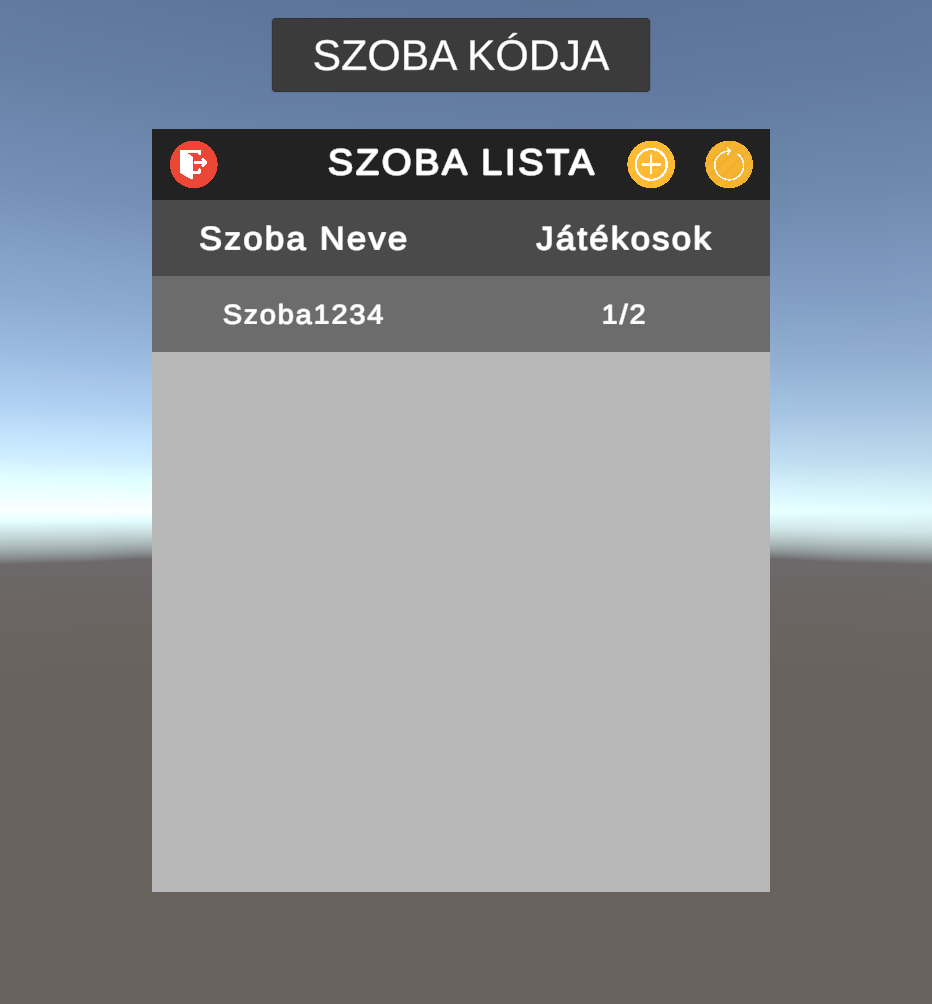
\includegraphics[width=0.8\textwidth]{lobbylist}
	\caption{A szobák listázása és létrehozása}
	\label{fig:lobby-list}
\end{figure}

A szobában a játékosok láthatják egymás nevét és státuszát (host/kliens). A host játékos indíthatja el a játékot, amikor mindkét játékos csatlakozott.

\begin{figure}[h]
	\centering
	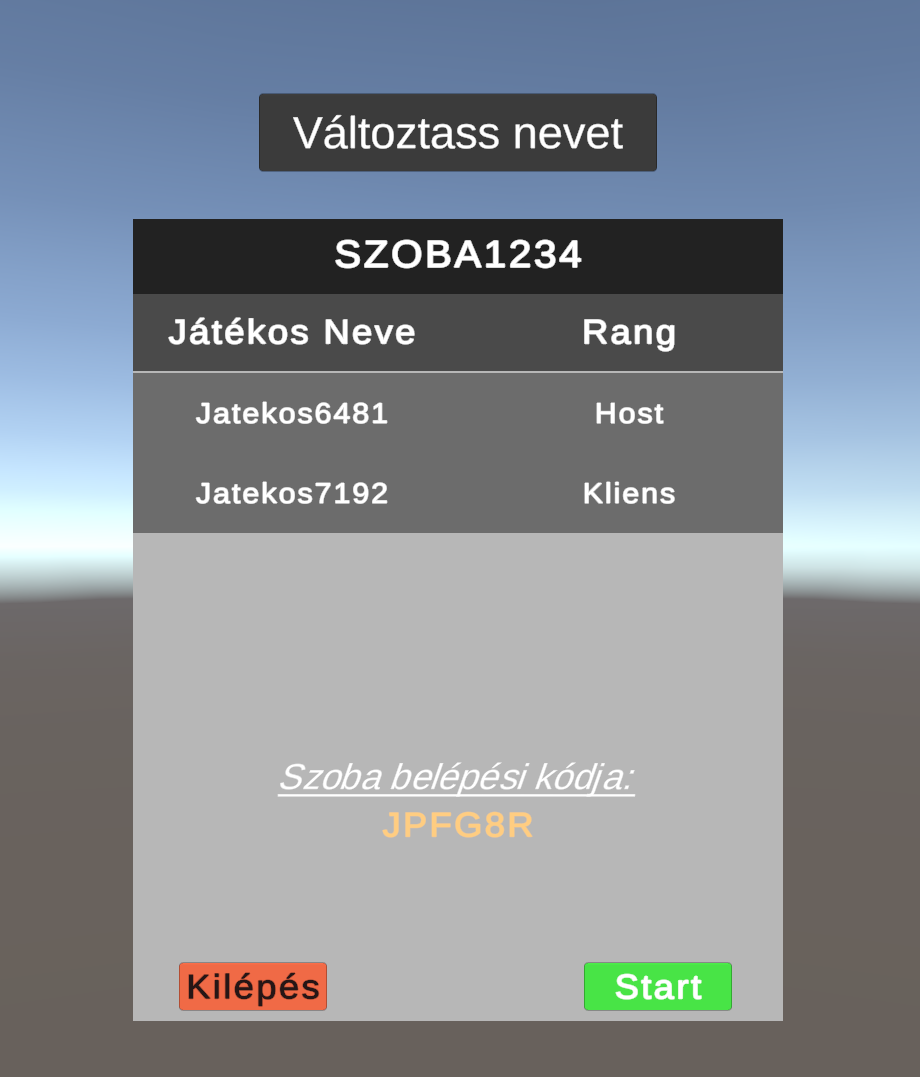
\includegraphics[width=0.8\textwidth]{lobby}
	\caption{Részletek a játékszobában}
	\label{fig:lobby-details}
\end{figure}

\subsection{Játékmenet}
A játék során a játéktábla 3D nézetben jelenik meg. A játékosok felváltva választhatnak gödröt a saját oldalukon kattintással. A program automatikusan végrehajtja a lépést, animálva a kövek mozgását.

\begin{figure}[h]
	\centering
	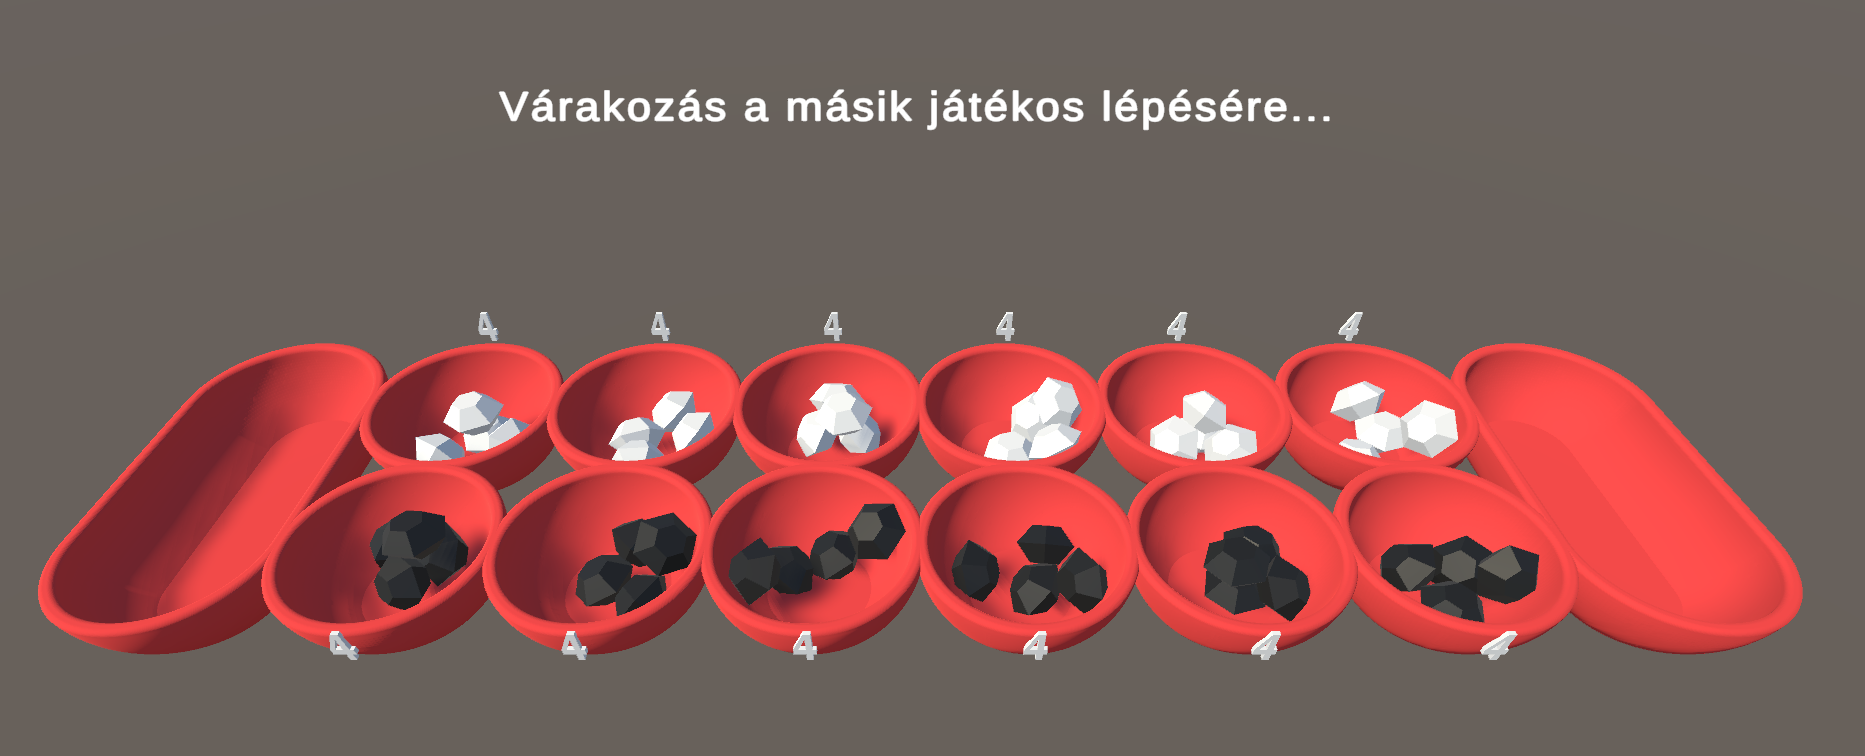
\includegraphics[width=0.8\textwidth]{gamestart}
	\caption{A játéktábla játék kezdetén}
	\label{fig:game-start}
\end{figure}

A játék állapotát jelző információk folyamatosan láthatók:
\begin{itemize}
	\item Az soron következő játékos jelzése
	\item A gödrökben lévő kövek száma
\end{itemize}

\section{Hibaelhárítás}

\subsection{Kapcsolódási problémák}
Ha problémák merülnek fel az online játék során:
\begin{itemize}
	\item Ellenőrizze az internetkapcsolatot
	\item Próbáljon újracsatlakozni a szobához
	\item Ha a probléma továbbra is fennáll, indítsa újra az alkalmazást
\end{itemize}

\subsection{Ismert hibák}
\begin{itemize}
	\item Ritkán előfordulhat, hogy a kövek mozgatásánál egy kő kiesik/két tároló közé esik.
	\item Egyes esetekben a játékos neve nem frissül ha a hoszt elindítja a játékot míg a név változtatás nem történt meg.
\end{itemize}

Ezen hibák általában nem befolyásolják a játék működését, és a következő körre vagy lépés után automatikusan javulnak.